\documentclass[12pt,a4paper,oneside]{article}

\usepackage[utf8]{inputenc}
\usepackage[portuguese]{babel}
\usepackage[T1]{fontenc}
\usepackage{amsmath}
\usepackage{amsfonts}
\usepackage{amssymb}
\usepackage{url}
\usepackage{graphicx}
\usepackage{caption}
\usepackage{subcaption}
\usepackage[table]{xcolor}

\newcommand{\lcc}{Lógica para Ciência da Computação }
\newcommand{\tc}{Teoria da Computação }
\newcommand{\curso}{\tc}
\newcommand{\sem}{2014.1 }

\author{\\Universidade Federal de Goiás (UFG) \\Bacharelado em Ciência da Computação 
\\ \curso \sem \\Prof. Esdras Lins Bispo Jr.}

\title{\sc \huge Instruções sobre a \\Avaliação pelos Pares}

\begin{document}

\maketitle

Avaliação pelos pares é quando indivíduos consideram quantidade, nível, valor, relevância, qualidade ou sucesso de um determinado resultado do aprendizado dos seus pares de ``{\it status}'' semelhantes \cite{topping}. Por exemplo, quando é enviado um artigo para um congresso, pesquisadores daquela área avaliam o artigo enviado. São pesquisadores avaliando pesquisadores. Praticamente toda a produção científica mundial está baseada neste tipo de avaliação.

Nas universidades e faculdades, a avaliação pelos pares vem sendo adotada com o propósito de extrair indicadores alternativos da aprendizagem desenvolvida pelo estudante. Universidades como Stanford \cite{stanford}, Cornell \cite{cornell}, Reading \cite{reading} e Leeds \cite{orsmond} já estão trabalhando ou pesquisando este formato de avaliação com os seus estudantes. Normalmente, a avaliação pelos pares é feita de forma suplementar (e não substitutiva) ao processo de avaliação já utilizado.

Este documento tem como propósito detalhar como será utilizada a avaliação pelos pares na disciplina de \curso \sem na Universidade Federal de Goiás, Câmpus Jataí. A Seção \ref{met} explanará sobre como será a metodologia da nossa avaliação. A Seção \ref{crit} apresentará os critérios de correção a ser utilizados. A Seção \ref{aval} explicará como será realizada a avaliação no {\sf Canvas} E, por fim, as referências utilizadas neste documento.

\section{Metodologia} \label{met}

Durante a disciplina de \curso, serão disponibilizadas várias listas de exercícios. Periodicamente, um ou dois exercícios serão escolhidos para serem avaliados. Cada exercício será avaliado pelos seguintes indivíduos:

	\begin{itemize}
		\item três outros estudantes;
		\item o professor.
	\end{itemize}

A pontuação será atribuída conforme a Equação (1), se o estudante for avaliado pelo professor
\begin{eqnarray}
	Pont & = & \dfrac{E_1 + E_2 + E_3 + P}{4}
\end{eqnarray}
e pela Equação (2), se o estudante não for avaliado pelo professor
\begin{eqnarray}
	Pont & = & \dfrac{E_1 + E_2 + E_3}{3}
\end{eqnarray}
em que:
\begin{itemize}
	\item $E_1$, $E_2$, $E_3$ são as três pontuações dadas por outros estudantes; e
	\item $P$ é a pontuação dada pelo professor.
\end{itemize}

O professor avaliará um grupo aleatório de $n$ alunos a cada exercício. A quantidade $n$ será proporcional ao tamanho da turma (por exemplo, 10\% da turma). O professor escolherá essa porcentagem a partir da avaliação do primeiro exercício.

\section{Ambiente Virtual de Aprendizagem} \label{crit}

O Ambiente Virtual de Aprendizagem (AVA) que utilizaremos será o {\sf Canvas} desenvolvido pela {\sf Instructure Inc.}\footnote{\url{http://www.instructure.com/}}. O {\sf Canvas} foi fundado em 2008 e já utilizado em mais de 400 escolas e universidades. O {\sf Canvas} pode ser acessado através de várias formas como computadores pessoais (\url{https://canvas.instructure.com/}) e dispositivos móveis (como celulares e {\it tablets}). Na Figura \ref{canvas}, podemos ver os vários logos utilizados pela AVA no {\it site}, {\sf Play Store} ({\sf Google}) e {\sf Apple Store}.

\begin{figure}[htb]
	\centering
	\begin{subfigure}[b]{0.3\textwidth}
		\centering
		
\includegraphics[width=\textwidth]{imagens/canvas.png}
		\caption{Site.}
		\label{canvasLogo}
	\end{subfigure}
	\begin{subfigure}[b]{0.3\textwidth}
		\centering
		
\includegraphics[width=0.5\textwidth]{imagens/canvasApp.png}
		\caption{{\sf Play Store}.}
		\label{canvasApp}
	\end{subfigure}
	\begin{subfigure}[b]{0.3\textwidth}
		\centering
		
\includegraphics[width=0.5\textwidth]{imagens/canvasIPhone.jpg}
		\caption{{\sf Apple Store}.}
		\label{canvasApple}
	\end{subfigure}
	\caption{Logotipo do {\sf Canvas}.}
	\label{canvas}
\end{figure}

\section{Como avaliar?} \label{aval}

Os critérios utilizados para a correção estarão disponíveis no {\sf Canvas}. No canto superior direito da janela de avaliação, haverá um link chamado {\bf Exibir protocolo} (ver Figura \ref{canvasProt}) que mostrará quais critérios devem ser utilizados e qual a pontuação devida de cada critério. Cada estudante deverá corrigir os exercícios de três outros estudantes seguindo os critérios estabelecidos.

\begin{figure}[htb]
	\centering
	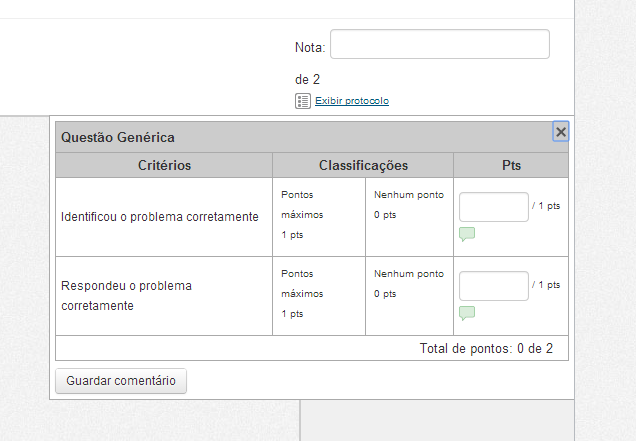
\includegraphics[width=.6\textwidth]{imagens/exibirProtocolo.png}
	\caption{Captura de tela do {\sf Canvas} exibindo o clique no {\it link} chamado {\bf Exibir protocolo}.}
	\label{canvasProt}
\end{figure}

Vamos supor que o protocolo estabelecido pelo professor seja conforme a Figura \ref{supProt}. O aluno terá que avaliar, para uma dada questão, os dois critérios do protocolo: (i) {\sf Identificou o problema corretamente?}; e (ii) {\sf Respondeu o problema corretamente?}. Para cada critério, é necessário fornecer uma classificação para o desempenho do colega. 

\begin{figure}[htb]
	\centering
	\begin{subfigure}[b]{0.4\textwidth}
		\centering
		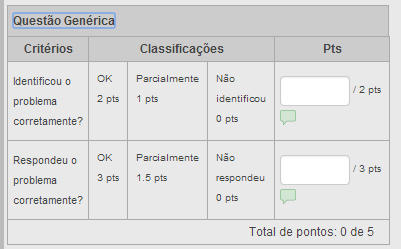
\includegraphics[width=\textwidth]{imagens/supostoProtocolo.png}
		\caption{Suposto protocolo.}
		\label{supProt}
	\end{subfigure}
	\begin{subfigure}[b]{0.4\textwidth}
		\centering
		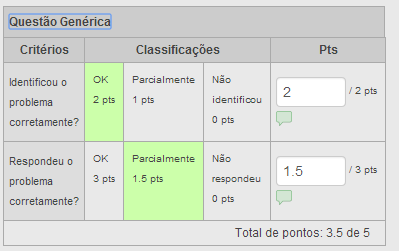
\includegraphics[width=\textwidth]{imagens/supostaAvaliacao.png}
		\caption{Suposta avaliação.}
		\label{supAval}
	\end{subfigure}
	\caption{Protocolos no {\sf Canvas}.}
	\label{sup}
\end{figure}

Por exemplo, imagine um aluno que para o critério (i) classificou o colega como ``OK'', e para o critério (ii) classificou-o como ``Parcialmente''. A pontuação final do colega seria {\sf 3.5/5.0} (3,5 de 5,0 pontos que poderiam ser obtidos). A Figura \ref{supAval} apresenta como ficaria a tela do {\sf Canvas} nesta situação.

\section{Considerações Importantes} \label{cons}

\begin{itemize}
	\item É necessário lembrar que depois de o aluno utilizar o protocolo, ele {\bf necessita} preencher o campo {\sf Nota:} (ver Figura \ref{canvasProt}) com a referida nota por ele classificada;
	\item O separador de decimais utilizado pelo sistema é o ponto (.), ao invés da vírgula (,) [por exemplo, quatro e meio tem que ser colocado como 4.5, ao invés de 4.5];
	\item Sempre que possível, coloque comentários sobre a classificação dada ao seu colega nesta questão (existe um balãozinho do lado de cada critério).
\end{itemize}

\begin{thebibliography}{9}

\footnotesize

\bibitem{cornell} Cornell University. {\bf Peer Assessment}. Acesso em 28 de fevereiro de 2014. Disponível em \url{http://www.cte.cornell.edu/teaching-ideas/assessing-student-} \url{learning/peer-assessment.html}.

\bibitem{stanford} Coursera Inc. {\bf How do peer assessments work?} Acesso em 28 de fevereiro de 2014. Disponível em \url{http://help.coursera.org/customer/portal/articles/1163294-how-do-peer-assessments-work-}

\bibitem{reading} Education Enhancement Unit, University of Exeter. {\bf Principles for using self and peer assessment}. Acesso em 28 de fevereiro de 2014. Disponível em \url{http://www.rea} \url{ding.ac.uk/internal/engageinfeedback/efb-PrinciplesForUsingSelfAndPeer} \url{Assessment.aspx}.

\bibitem{orsmond} Orsmond, P. {\bf Self and Peer-Assessment: Guidance in Practice in the Biosciences}. Leeds: Centre for
Bioscience, The Higher Education Academy, 2004.

\bibitem{topping} Topping, K. {\it Peer assessment between students in colleges and universities}. In {\bf Review of Educational Research}. 68.3, 249-276 p, 1998.

\end{thebibliography}

\end{document}